\documentclass[10pt]{beamer}

\usepackage{color}
\usepackage{listings}

\usetheme{Hannover}
\usefonttheme{serif}
\usecolortheme{seagull}
\beamertemplatenavigationsymbolsempty
\setbeamertemplate{blocks}[rounded][shadow=false]

\definecolor{Blue}{rgb}{0.0, 0.0, 0.8}
\definecolor{DarkGreen}{rgb}{0.0, 0.5, 0.0}
\definecolor{DarkGray}{rgb}{0.5, 0.5, 0.5}
\definecolor{Gray}{rgb}{0.8, 0.8, 0.8}
\definecolor{Orange}{rgb}{0.8, 0.5, 0.0}
\definecolor{White}{rgb}{1.0, 1.0, 1.0}

\lstset{
  basicstyle=\ttfamily\footnotesize,
  breakatwhitespace=false,
  breaklines=true,
  captionpos=b,
  commentstyle=\color{DarkGreen},
  escapeinside={\%*}{*)},
  extendedchars=true,
  frameshape={RYR}{Y}{Y}{RYR},
  keepspaces=true,
  keywordstyle=\color{Blue},
  numbers=left,
  numbersep=6pt,
  numberstyle=\tiny\color{DarkGray},
  rulecolor=\color{Gray},
  showspaces=false,
  showstringspaces=false,
  showtabs=false,
  stepnumber=2,
  stringstyle=\color{Orange},
  tabsize=2
}

\title{Who's Hacking Who?}
\subtitle{
  From Russia with Love
  \vspace{0.5cm}
  \\
  
\includegraphics[height=3cm,keepaspectratio]{hackers.jpg}
  \\
  \scriptsize{\emph{Hackers - 1995}}
}
\author[Barry, Bol]{D.~Barry\inst{1} \and L.Bol\inst{1}}
\institute{
  \inst{1}
  Computer Science Society
  \\
  University of Hertforshire
}
\date{October, 2016}
\subject{Computer Science}

\begin{document}
  %%%%%%%%%%%%%%%%%%%%%%%%%%%%%%%%%%%%%
  % Title
  %%%%%%%%%%%%%%%%%%%%%%%%%%%%%%%%%%%%%
  \frame{\titlepage}
  \begin{frame}
    \frametitle{Table of Contents}
    \begin{block}{}
      \vspace{0.5cm}
      \tableofcontents
      \vspace{0.5cm}
    \end{block}
  \end{frame}
  %%%%%%%%%%%%%%%%%%%%%%%%%%%%%%%%%%%%%
  % Introduction
  %%%%%%%%%%%%%%%%%%%%%%%%%%%%%%%%%%%%%
  \section[Intro]{Introduction}
  \begin{frame}
    \frametitle{Credentials}
    \centering
    \begin{tabular}{| r | c | c |}
      \hline
                 & Daniel Barry                                            & Lukasz Bol     \\
                 & 
\includegraphics[width=2cm,keepaspectratio]{dbarry.jpg} & 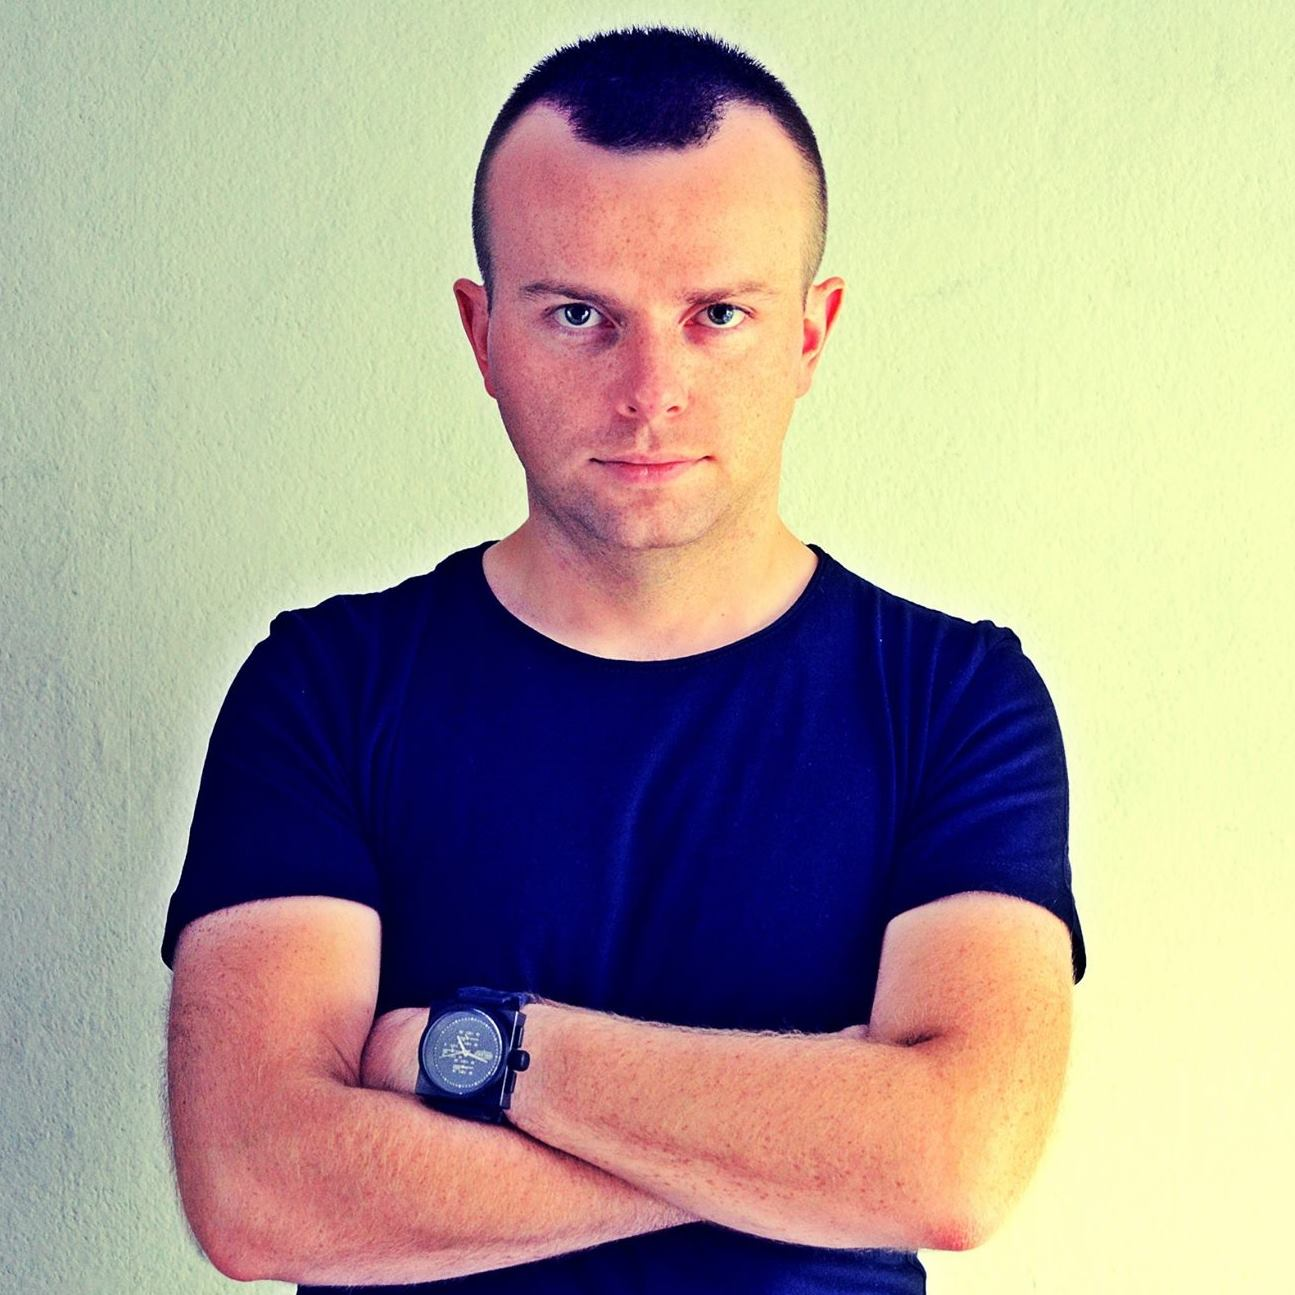
\includegraphics[width=2cm,keepaspectratio]{lbol.jpg} \\
      \hline
      From       & Essex, UK                                               & Lodz, Poland                                          \\
      Study      & MSc                                                     & BSc (3rd Year)                                        \\
      Society    & Mentor                                                  & Chair                                                 \\
      Speciality & AI                                                      & IoT                                                   \\
      University & (Past) Student Rep                                      & (Past) Student Rep                                    \\
                 & PAL Leader                                              & PAL Leader                                            \\
                 & Student Proctor                                         & Student Proctor                                       \\
      Work Exp   & Visteon                                                 & Self-employed DJ                                      \\
      \hline
    \end{tabular}
  \end{frame}
  \begin{frame}
    \frametitle{Previous Projects}
    \centering
    \begin{tabular}{p{4cm} p{4cm}}
      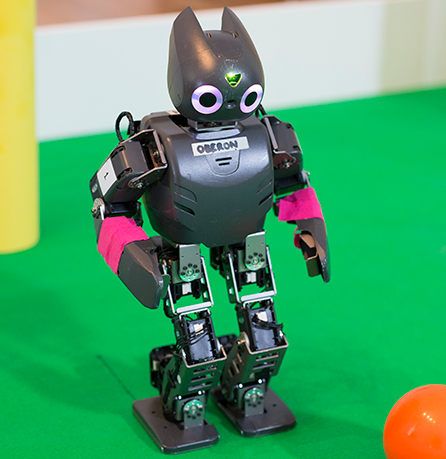
\includegraphics[width=2cm,keepaspectratio]{robocup.png}     &
      
\includegraphics[width=2cm,keepaspectratio]{netizens.png}   \\
      RoboCup - \emph{Football playing robots}                     &
      Netizens - \emph{UH hacking group}                          \\
      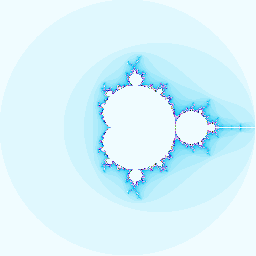
\includegraphics[width=2cm,keepaspectratio]{mandelbrot.png}  &
      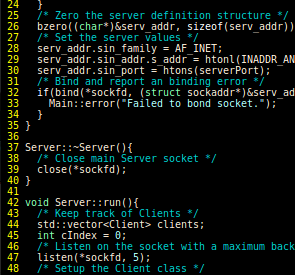
\includegraphics[width=2cm,keepaspectratio]{palproctor.png} \\
      General Programming - \emph{Too much to mention!}            &
      PAL \& Proctoring - \emph{Mentoring students}               \\
    \end{tabular}
  \end{frame}
  %%%%%%%%%%%%%%%%%%%%%%%%%%%%%%%%%%%%%
  % Aims
  %%%%%%%%%%%%%%%%%%%%%%%%%%%%%%%%%%%%%
  \section[Aims]{Aims}
  \begin{frame}
    \frametitle{Aims Today}
    \textbf{TODO:} Write this text.
  \end{frame}
  \begin{frame}
    \frametitle{Aims Over Time}
    \textbf{TODO:} Write this text.
  \end{frame}
  %%%%%%%%%%%%%%%%%%%%%%%%%%%%%%%%%%%%%
  % Development
  %%%%%%%%%%%%%%%%%%%%%%%%%%%%%%%%%%%%%
  \section[Dev]{Development}
  \begin{frame}[fragile=singleslide]
    \frametitle{API}
    \begin{lstlisting}[caption=Java Hello World,language=Java]
/**
 * main()
 *
 * The main entry point into the program.
 *
 * @param args The arguments passed via the command line.
 **/
public static void main(String[] args){
  System.out.println("Hello World");
}
    \end{lstlisting}
  \end{frame}
  %%%%%%%%%%%%%%%%%%%%%%%%%%%%%%%%%%%%%
  % Conclusion
  %%%%%%%%%%%%%%%%%%%%%%%%%%%%%%%%%%%%%
  \section[End]{Conclusion}
  \begin{frame}
    \frametitle{Achievements}
    \textbf{TODO:} Write this text.
  \end{frame}
  \begin{frame}
    \frametitle{Wrapping Up}
    \begin{block}{}
      \centering
      Any questions?
    \end{block}
  \end{frame}
\end{document}
